\documentclass[11pt,a4paper]{article}

% Packages
\usepackage[utf8]{inputenc}
\usepackage[spanish, es-tabla, es-lcroman]{babel}
\usepackage{caption}
\usepackage{listings}
\usepackage{adjustbox}
\usepackage{amssymb, amsmath, amsthm}
\usepackage[margin=1in]{geometry}
\usepackage[shortlabels]{enumitem}
\usepackage{xcolor}
\usepackage{soul}
\usepackage{listings}
\usepackage{graphicx}
\usepackage{float}

% Meta
\title{Práctica 1: Estudio de la eficiencia}
\author{José Antonio Álvarez Ocete - Norberto Fernández de la Higuera \\ Javier Gálvez Obispo - Yábir García Benchakhtir }
\date{\today}

% Custom
\providecommand{\abs}[1]{\lvert#1\rvert}
\setlength\parindent{0pt}
\definecolor{Light}{gray}{.90}
\newcommand\ddfrac[2]{\frac{\displaystyle #1}{\displaystyle #2}}

% Listings
\lstset{literate=   % listings config
  {á}{{\'a}}1 {é}{{\'e}}1 {í}{{\'i}}1 {ó}{{\'o}}1 {ú}{{\'u}}1
  {Á}{{\'A}}1 {É}{{\'E}}1 {Í}{{\'I}}1 {Ó}{{\'O}}1 {Ú}{{\'U}}1
  {à}{{\`a}}1 {è}{{\`e}}1 {ì}{{\`i}}1 {ò}{{\`o}}1 {ù}{{\`u}}1
  {À}{{\`A}}1 {È}{{\'E}}1 {Ì}{{\`I}}1 {Ò}{{\`O}}1 {Ù}{{\`U}}1
  {ä}{{\"a}}1 {ë}{{\"e}}1 {ï}{{\"i}}1 {ö}{{\"o}}1 {ü}{{\"u}}1
  {Ä}{{\"A}}1 {Ë}{{\"E}}1 {Ï}{{\"I}}1 {Ö}{{\"O}}1 {Ü}{{\"U}}1
  {â}{{\^a}}1 {ê}{{\^e}}1 {î}{{\^i}}1 {ô}{{\^o}}1 {û}{{\^u}}1
  {Â}{{\^A}}1 {Ê}{{\^E}}1 {Î}{{\^I}}1 {Ô}{{\^O}}1 {Û}{{\^U}}1
  {œ}{{\oe}}1 {Œ}{{\OE}}1 {æ}{{\ae}}1 {Æ}{{\AE}}1 {ß}{{\ss}}1
  {ű}{{\H{u}}}1 {Ű}{{\H{U}}}1 {ő}{{\H{o}}}1 {Ő}{{\H{O}}}1
  {ç}{{\c c}}1 {Ç}{{\c C}}1 {ø}{{\o}}1 {å}{{\r a}}1 {Å}{{\r A}}1
  {€}{{\EUR}}1 {£}{{\pounds}}1 {ñ}{{\~{n}}}1
}

\lstset{    %listings config
	language=C++,
	belowcaptionskip=1\baselineskip,
	breaklines=true,
	frame=L,
	xleftmargin=0.1in,
	%otherkeywords={},
	showstringspaces=false,
	backgroundcolor=\color{white},
	basicstyle=\footnotesize\ttfamily,
	keywordstyle=\bfseries\color{purple!90!black},
	commentstyle=\itshape\color{gray!85!},
	identifierstyle=\color{blue!80!black},
	stringstyle=\color{green!60!black},
}

\begin{document}

\maketitle

\section{Introducción}

En esta práctica realizaremos un estudio de la eficiencia tanto empírica como híbrida de los algoritmos propuestos en el guión de prácticas. Siguiendo dicho guión, realizaremos distintas gráficas mostrando el trabajo realizado y expondremos diversos resultados para los distintos miembros del equipo.

Adjunto a esta memoria se entregarán los datos tomados así como las gráficas generadas a partir de los mismos.

\section{Informe de la eficiencia}

Los algoritmos propuestos para el estudio de la eficiencia son los siguientes:

\begin{table}[H]
	\centering
	\caption{Algoritmos a estudiar.}
	\label{my-label}
	\begin{tabular}{ll}
		Algoritmo & Eficiencia   \\
		burbuja   & $O(n^2)$     \\
		inserción & $O(n^2)$     \\
		selección & $O(n^2)$     \\
		mergesort & $O(n log n)$ \\
		quicksort & $O(n log n)$ \\
		heapsort  & $O(n log n)$ \\
		floyd     & $O(n^3)$     \\
		hanoi     & $O(2^n)$
	\end{tabular}
\end{table}

Para el estudio de estos, cada miembro del grupo ha utilizado un equipo distinto:

\begin{itemize}
\item En el caso de Yabir se ha utilizado un Intel Pentium G3258 con 2 núcleos a 3.2GHz,
  8GB de RAM y el sistema operativo Linux Mint 18.3 Sylvia x86 64.
\item Javier por su parte, ha utilizado un i5-6200U con 4 núcleos a 2.3GHz, 8GB de RAM
y ubuntu 16 LTS de 64 bits como sistema operativo.
\item Por otro lado Jose Antonio ha utilizado un i7-5500 con 4 núcleos a 2.4GHz, 8GB de RAM
  y ubuntu 16 LTS de 64 bits.
\item Y por último Norberto ha utilizado un i5-4590 con 4 núcleos a 3.3GHz, 8GB de RAM y
ubuntu 16 LTS de 64 bits.
  
\end{itemize}

\subsection{Algoritmos de orden cuadrático}

En primer lugar realizamos un estudio teórico de la eficiencia. Como se vió en el guión de prácticas, la eficiencia teórica del algoritmo \emph{burbuja} es de:

$$\frac{a}{2} n^2 - \frac{3a}{2} n + a \in O(n^2)$$

Donde $a$ es una constante que acota el interior del bucle.

Repetimos un proceso análogo al realizado para el algóritmo de burbuja estudiando \textbf{selección} para el siguiente código:

\begin{lstlisting}
static void seleccion_lims(int T[], int inicial, int final) {
	int i, j, indice_menor;
	int menor, aux;
	for (i = inicial; i < final - 1; i++) {
		indice_menor = i;
		menor = T[i];
		for (j = i; j < final; j++) {
			if (T[j] < menor) {
				indice_menor = j;
				menor = T[j];
			}
		}
		aux = T[i];
		T[i] = T[indice_menor];
		T[indice_menor] = aux;
	};
}
\end{lstlisting}

Acotamos el contenido del bucle for anindado por la constante $a_1$ y
las operaciones del bucle exterior por la constante $a_2$.  De esta
manera el análisis de la eficiencia sería el soguiente.

\begin{equation}
  \begin{aligned}
    \sum_{i=0}^{n-1}\left[a_2 + \sum_{j=i}^n{a_1}\right] &= \sum_{i=0}^{n-1}\left[a_2+a_1\sum_{j=i}^{n}1\right]  \\
    &= \sum_{i=0}^{n-1}a_2 + a_1 \sum_{i=0}^{n}\sum_{j=i}^{n-1}1 \\
    &= a_2\sum_{i=0}^{n-1}1 + a_1 \sum_{i=0}^{n}(n-i)
  \end{aligned}
\end{equation}

de la primera sumatoria extraemos $b(n-1)$ y ahora procedemos a analizar la segunda:

\begin{equation}
  \begin{aligned}
    a\sum_{i=0}^{n-1}(n-i) &= a_1\left[\sum_{i=0}^{n}n - \sum_{i=0}^{n}i\right]  \\
    &= an^2 - a \frac{(n+1)n}{2} \\
    &= an^2- \frac{an^2}{2} - \frac{an}{2}
  \end{aligned}
\end{equation}

Sumando ambas expresiones obtenemos:

$$\frac{an^2}{2} - \frac{an}{2}+ b(n-1) = \frac{a}{2}n^2+\frac{b-a}{2}n - b \in O(n^2)$$



Para el caso de \textbf{inserción} tenemos el siguiente algoritmo:

\begin{lstlisting}
static void insercion_lims(int T[], int inicial, int final)
{
	int i, j;
	int aux;
	for (i = inicial + 1; i < final; i++) {
		j = i;
		while ((T[j] < T[j-1]) && (j > 0)) {
			aux = T[j];
			T[j] = T[j-1];
			T[j-1] = aux;
			j--;
		};
	};
}
\end{lstlisting}

Manteniendo la notación utilizado y utilizando un razonamiento similiar al anterior obtenemos:

$$\sum_{i=0}^{n} \sum_{j=i}^{n} a = ... = a \cdot (\frac{n^2}{2} + 2n) \in O(n^2)$$

Realizado el estudio teórico sobre los tres algoritmos, ejecutamos y utilizamos \emph{gnuplot} para obtener un ajuste de los datos obtenidos. Representamos ahora los datos obtenidos junto a una comparativa gráfica de los tiempos generados para los distintos miembros del grupo.

\begin{table}[h]
	\centering
	\caption{Burbuja}
	\begin{tabular}{ | c | c  | c | c | c | }
		\hline
		Tama\~no & Jose Antonio & Yabir & Javier & Norberto\\
		\hline
		1000	&	0.002102	&	0.004246	&	0.004012	&	0.001311	\\
		2000	&	0.008624	&	0.008201	&	0.015366	&	0.007047	\\
		3000	&	0.019598	&	0.019307	&	0.015748	&	0.017844	\\
		4000	&	0.036247	&	0.034225	&	0.027918	&	0.022229	\\
		5000	&	0.059415	&	0.056845	&	0.051099	&	0.039783	\\
		6000	&	0.089915	&	0.088076	&	0.077024	&	0.061048	\\
		7000	&	0.126946	&	0.120856	&	0.114816	&	0.088834	\\
		8000	&	0.174056	&	0.161862	&	0.156521	&	0.121957	\\
		9000	&	0.221849	&	0.210286	&	0.207334	&	0.16015	\\
		10000	&	0.279818	&	0.264146	&	0.264914	&	0.207358	\\
		11000	&	0.341537	&	0.323677	&	0.328079	&	0.25534	\\
		12000	&	0.410517	&	0.394902	&	0.401309	&	0.30851	\\
		13000	&	0.487268	&	0.463354	&	0.475421	&	0.368633	\\
		14000	&	0.574468	&	0.541129	&	0.562932	&	0.434771	\\
		15000	&	0.669231	&	0.628463	&	0.652525	&	0.50592	\\
		16000	&	0.761777	&	0.718559	&	0.756564	&	0.579439	\\
		17000	&	0.859512	&	0.814468	&	0.860402	&	0.661685	\\
		18000	&	0.972132	&	0.919391	&	0.970756	&	0.751912	\\
		19000	&	1.08788	&	1.03422	&	1.08355	&	0.841164	\\
		20000	&	1.21375	&	1.14783	&	1.21362	&	0.944326	\\
		21000	&	1.35448	&	1.27545	&	1.35594	&	1.04575	\\
		22000	&	1.4721	&	1.39817	&	1.50011	&	1.15543	\\
		23000	&	1.6226	&	1.53151	&	1.65828	&	1.27277	\\
		24000	&	1.76133	&	1.67702	&	1.81174	&	1.3934	\\
		25000	&	1.92358	&	1.81403	&	1.98219	&	1.51766	\\
		\hline
	\end{tabular}
\end{table}

\begin{figure}[H]
	\centering
	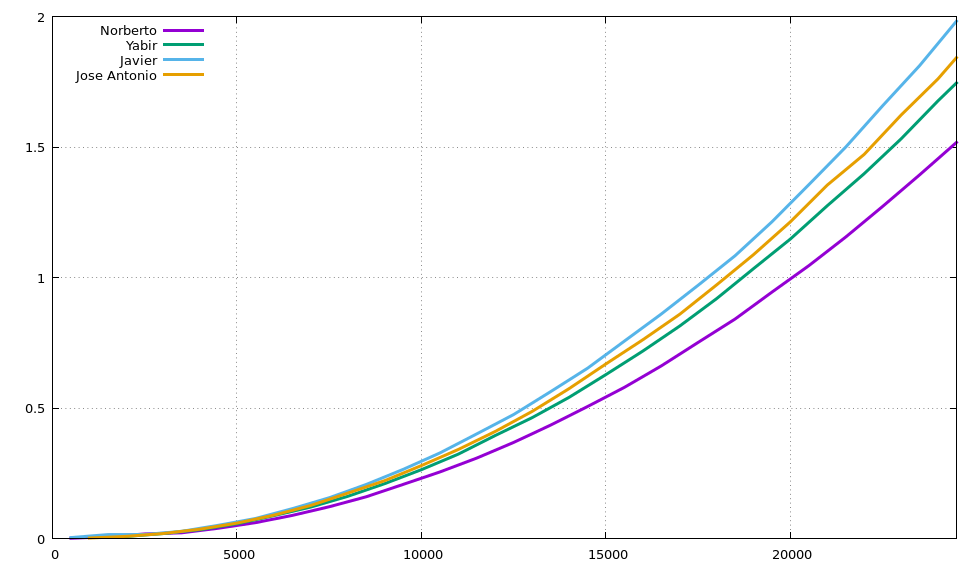
\includegraphics[width=0.8\textwidth]{../plots/burbuja}
	\caption{Comparativa de la eficiencia empírica del algoritmo $burbuja$.}
\end{figure}

\begin{table}[h]
	\centering
	\caption{Inserción}
	\begin{tabular}{ | c | c  | c | c | c | }
		\hline
		Tama\~no & Jose Antonio & Yabir & Javier & Norberto\\
		\hline
		1000	&	0.0012	&	0.00112	&	0.000545	&	0.001092	\\
		2000	&	0.004572	&	0.004292	&	0.003054	&	0.003372	\\
		3000	&	0.010898	&	0.009728	&	0.008701	&	0.007137	\\
		4000	&	0.018749	&	0.017294	&	0.015705	&	0.013268	\\
		5000	&	0.029047	&	0.026957	&	0.024028	&	0.019037	\\
		6000	&	0.040956	&	0.038868	&	0.036763	&	0.028616	\\
		7000	&	0.055705	&	0.052248	&	0.050062	&	0.039232	\\
		8000	&	0.072807	&	0.068156	&	0.068483	&	0.053949	\\
		9000	&	0.092916	&	0.086587	&	0.08547	&	0.067547	\\
		10000	&	0.113404	&	0.107304	&	0.109743	&	0.087403	\\
		11000	&	0.137771	&	0.130252	&	0.131087	&	0.103835	\\
		12000	&	0.164464	&	0.15566	&	0.155903	&	0.123986	\\
		13000	&	0.193596	&	0.182503	&	0.182363	&	0.147122	\\
		14000	&	0.228399	&	0.212983	&	0.216041	&	0.17068	\\
		15000	&	0.257807	&	0.243724	&	0.25058	&	0.196732	\\
		16000	&	0.291294	&	0.2767	&	0.297828	&	0.225098	\\
		17000	&	0.328677	&	0.309732	&	0.32026	&	0.255474	\\
		18000	&	0.367407	&	0.346489	&	0.363618	&	0.288498	\\
		19000	&	0.407266	&	0.387793	&	0.400226	&	0.319619	\\
		20000	&	0.467829	&	0.432006	&	0.446305	&	0.355745	\\
		21000	&	0.500632	&	0.479765	&	0.508203	&	0.394738	\\
		22000	&	0.545645	&	0.524347	&	0.54851	&	0.433908	\\
		23000	&	0.595075	&	0.569582	&	0.601286	&	0.475005	\\
		24000	&	0.659751	&	0.620089	&	0.678724	&	0.517875	\\
		25000	&	0.711745	&	0.675667	&	0.702348	&	0.562875	\\
		\hline
	\end{tabular}
\end{table}

\begin{figure}[H]
	\centering
	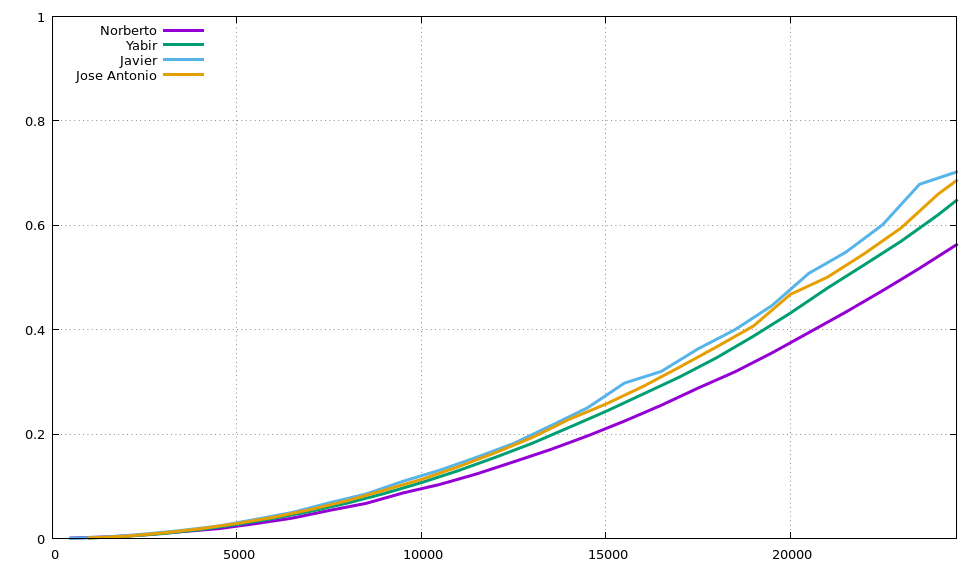
\includegraphics[width=0.8\textwidth]{../plots/insercion}
	\caption{Comparativa de la eficiencia empírica del algoritmo $insercion$.}
\end{figure}

\begin{table}[h]
	\centering
	\caption{Selección}
	\begin{tabular}{ | c | c  | c | c | c | }
		\hline
		Tama\~no & Jose Antonio & Yabir & Javier & Norberto\\
		\hline
		1000	&	0.00143505	&	0.00135595	&	0.00046005	&	0.00035719	\\
		2000	&	0.00561393	&	0.00524505	&	0.00340335	&	0.00261264	\\
		3000	&	0.012424	&	0.011705	&	0.009438	&	0.007685	\\
		4000	&	0.022427	&	0.020711	&	0.018861	&	0.016741	\\
		5000	&	0.034595	&	0.03227	&	0.03064	&	0.023002	\\
		6000	&	0.049521	&	0.046363	&	0.045548	&	0.034087	\\
		7000	&	0.067441	&	0.062962	&	0.062655	&	0.047873	\\
		8000	&	0.088587	&	0.082298	&	0.084243	&	0.063287	\\
		9000	&	0.111141	&	0.104299	&	0.107134	&	0.081399	\\
		10000	&	0.137052	&	0.128745	&	0.133317	&	0.103103	\\
		11000	&	0.166555	&	0.156038	&	0.162335	&	0.125322	\\
		12000	&	0.198069	&	0.185971	&	0.194576	&	0.149912	\\
		13000	&	0.231342	&	0.218305	&	0.230486	&	0.17692	\\
		14000	&	0.269093	&	0.253628	&	0.266774	&	0.20509	\\
		15000	&	0.308691	&	0.291057	&	0.308797	&	0.236309	\\
		16000	&	0.350138	&	0.331193	&	0.352636	&	0.271882	\\
		17000	&	0.400754	&	0.374365	&	0.39707	&	0.306598	\\
		18000	&	0.443237	&	0.419854	&	0.449266	&	0.343751	\\
		19000	&	0.495745	&	0.469411	&	0.500206	&	0.384171	\\
		20000	&	0.549374	&	0.518467	&	0.555784	&	0.426748	\\
		21000	&	0.603962	&	0.571629	&	0.614922	&	0.471934	\\
		22000	&	0.660961	&	0.62718	&	0.67396	&	0.521653	\\
		23000	&	0.722891	&	0.68739	&	0.737981	&	0.571422	\\
		24000	&	0.795483	&	0.747746	&	0.801045	&	0.621192	\\
		25000	&	0.861366	&	0.81211	&	0.879008	&	0.677699	\\
		\hline
	\end{tabular}
\end{table}

\begin{figure}[H]
	\centering
	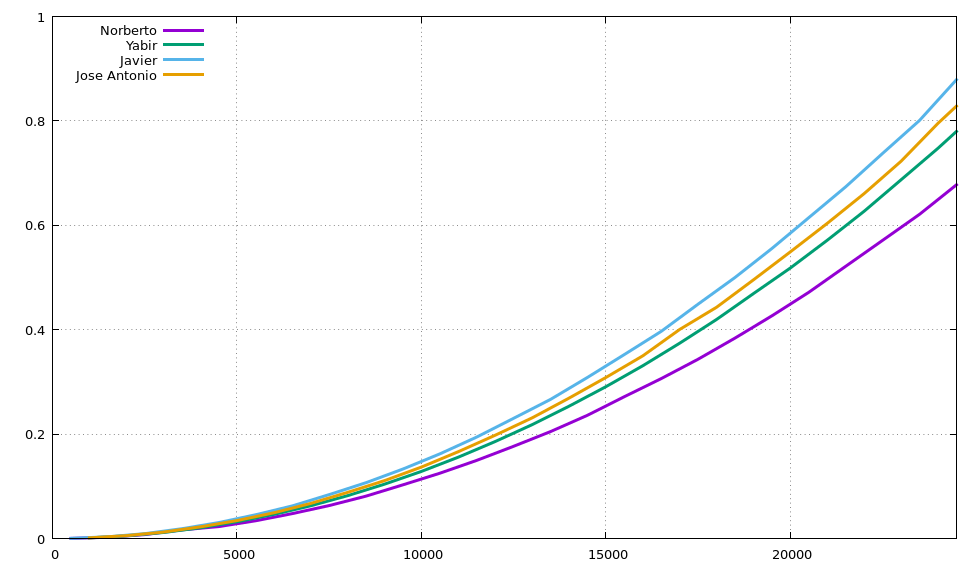
\includegraphics[width=0.8\textwidth]{../plots/seleccion}
	\caption{Comparativa de la eficiencia híbridia del algoritmo \emph{selección}.}
\end{figure}

\subsection{Algoritmos de orden n - logarítimico}

De nuevo comencemos realizando un estudio teórico. Como se vió en el
guión de prácticas, la eficiencia teórica de el algoritmo
\emph{mergesort} es de:

$$c_1n + c_2nlog_2(n) \in O(nlog_2(n))$$

Para el caso de \textbf{heapsort} tenemos el siguiente algoritmo:

\begin{lstlisting}
static void heapsort(int T[], int num_elem) {
	int i;
	for (i = num_elem/2; i >= 0; i--)
		reajustar(T, num_elem, i);
	for (i = num_elem - 1; i >= 1; i--) {
		int aux = T[0];
		T[0] = T[i];
		T[i] = aux;
		reajustar(T, i, 0);
	}
}

static void reajustar(int T[], int num_elem, int k) {
	int j;
	int v;
	v = T[k];
	bool esAPO = false;
	while ((k < num_elem/2) && !esAPO) {
		j = k + k + 1;
		if ((j < (num_elem - 1)) && (T[j] < T[j+1]))
			j++;
		if (v >= T[j])
			esAPO = true;
		T[k] = T[j];
		k = j;
	}
	T[k] = v;
}
\end{lstlisting}

Estudiaremos en primer lugar la eficiencia de la función
$Reajustar(k)$ que denotaremos por $R(k)$. Si nos fijamos en la
primera línea del bucle, en cada iteración multiplicamos $k \cdot
2$. Por lo tanto, si acotamos el interior del bucle por una constante
$c_1$ y $ t = n-k$:

$$R(n-k) = R(\frac{n-k}{2}) + c_1 \leftrightarrow R(t) = R(\frac{t}{2}) + c_1$$

Aplicando el cambio de variable $t = 2^m \leftrightarrow log_2 t = m$:

$$R(2^m) = R(2^{m-1}) + c_1$$

Denotando $R(2^m) = X_m$ obtenemos una ecuación en recurrencia:

$$X_m = X_{m-1} + c_1$$

Cuya solución es:

$$X_m = c_2 + c_1 * m$$

Donde $c_2$ es otra constance. Deshaciendo el cambio de variable obtenemos finalmente:

$$R(2^m) = R(t) = c_2 + c_1 * log_2(t) \in O(log(n))$$

A partir de la eficiencia de la función \textbf{Reajustar} es relativamente sencillo obtener la del algoritmo completo:

$$\sum_{i=0}^{n/2} R(i) + \sum_{i=1}^{n-1} (R(i) + c_3) $$

Como el logarítmo es una función creciente, acotamos los valores interiores de los bucles por el mayor valor alcanzado:

$$\sum_{i=0}^{n/2} R(i) + \sum_{i=1}^{n-1} (R(i) + c_3) \leq \sum_{i=0}^{n/2} R(n/2) + \sum_{i=1}^{n-1} (R(n-1) + c_3) = $$

$$= (n/2) \cdot R(n/2 + 1) + (n-1) \cdot R(n - 1) + c_3(n-1) = $$

$$= (n/2) \cdot R(n/2 + 1) + (n-1) \cdot R(n - 1) + c_3(n-1)$$

Como el orden de eficiencia de \textbf{Reajustar} es de $O(log(n))$, podemos concluir que el algoritmo tiene una eficiencia de $O(nlog(n))$

Realizado el estudio teórico sobre los tres algoritmos, ejecutamos y utilizamos \emph{gnuplot} para obtener un ajuste de los datos obtenidos. Adjuntamos a continuación las tablas con los datos obtenidos y una comparativa gráfica entre los distintos miembros del grupo.

\begin{table}[h]
	\centering
	\caption{Mergesort}
	\begin{tabular}{ | c | c  | c | c | c | }
		\hline
		Tama\~no & Jose Antonio & Yabir & Javier & Norberto\\
		\hline
		1000	&	0.000124104	&	0.000117755	&	6.0321e-05	&	5.8705e-05	\\
		2000	&	0.000275885	&	0.000265505	&	0.000264315	&	0.00020683	\\
		3000	&	0.000542727	&	0.000509884	&	0.000422699	&	0.00034141	\\
		4000	&	0.000609759	&	0.000580912	&	0.000544557	&	0.00042617	\\
		5000	&	0.000863075	&	0.000807877	&	0.000770273	&	0.00060328	\\
		6000	&	0.00112694	&	0.00107341	&	0.00103855	&	0.000831745	\\
		7000	&	0.00108948	&	0.00103389	&	0.00104633	&	0.00081689	\\
		8000	&	0.00132059	&	0.00124508	&	0.00127586	&	0.00099898	\\
		9000	&	0.00157088	&	0.00147816	&	0.00151632	&	0.00117791	\\
		10000	&	0.00184154	&	0.00174622	&	0.0017806	&	0.00138862	\\
		11000	&	0.002336	&	0.002063	&	0.002145	&	0.00161601	\\
		12000	&	0.002444	&	0.002352	&	0.002469	&	0.00186474	\\
		13000	&	0.002182	&	0.002076	&	0.003022	&	0.0021405	\\
		14000	&	0.002381	&	0.002313	&	0.002943	&	0.0018621	\\
		15000	&	0.002652	&	0.002485	&	0.002731	&	0.00202306	\\
		16000	&	0.002897	&	0.002708	&	0.003017	&	0.00221986	\\
		17000	&	0.003225	&	0.003018	&	0.003823	&	0.00242854	\\
		18000	&	0.003396	&	0.00331	&	0.003572	&	0.00263394	\\
		19000	&	0.003662	&	0.003453	&	0.003812	&	0.00285428	\\
		20000	&	0.003948	&	0.00379	&	0.004124	&	0.00308117	\\
		21000	&	0.004238	&	0.004064	&	0.004693	&	0.00331664	\\
		22000	&	0.004599	&	0.004262	&	0.005656	&	0.00356593	\\
		23000	&	0.005129	&	0.004612	&	0.005114	&	0.00382874	\\
		24000	&	0.00519	&	0.004959	&	0.005216	&	0.004356	\\
		25000	&	0.005524	&	0.005205	&	0.005718	&	0.00434365	\\
		\hline
	\end{tabular}
\end{table}

\begin{figure}[H]
	\centering
	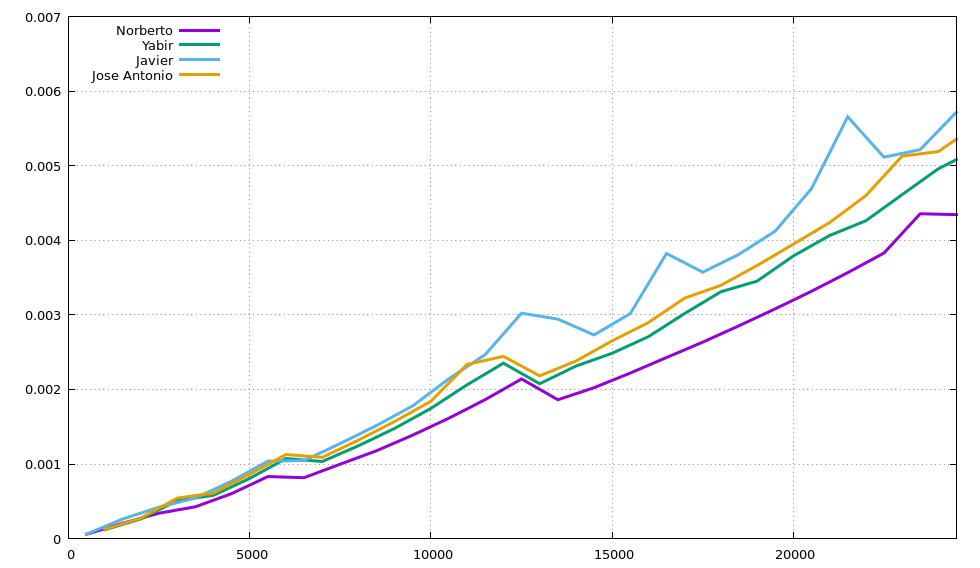
\includegraphics[width=0.8\textwidth]{../plots/mergesort}
	\caption{Comparativa de la eficiencia empírica del algoritmo $mergesort$.}
\end{figure}

\begin{table}[h]
	\centering
	\caption{Quicksort}
	\begin{tabular}{ | c | c  | c | c | c | }
		\hline
		Tama\~no & Jose Antonio & Yabir & Javier & Norberto\\
		\hline
		1000	&	9.5e-05	&	8.7e-05	&	5.8e-05	&	3.5e-05	\\
		2000	&	0.000235	&	0.000187	&	0.000254	&	0.00012	\\
		3000	&	0.000345	&	0.000294	&	0.000343	&	0.000235	\\
		4000	&	0.000506	&	0.000394	&	0.00061	&	0.000299	\\
		5000	&	0.000624	&	0.000534	&	0.000767	&	0.000436	\\
		6000	&	0.000812	&	0.000616	&	0.000732	&	0.000527	\\
		7000	&	0.000958	&	0.000727	&	0.000871	&	0.000629	\\
		8000	&	0.001056	&	0.000843	&	0.001239	&	0.000741	\\
		9000	&	0.001065	&	0.00097	&	0.001219	&	0.000865	\\
		10000	&	0.001216	&	0.001065	&	0.001331	&	0.000993	\\
		11000	&	0.001258	&	0.001219	&	0.001487	&	0.001072	\\
		12000	&	0.001415	&	0.001415	&	0.001637	&	0.001457	\\
		13000	&	0.001679	&	0.001446	&	0.001801	&	0.00144	\\
		14000	&	0.001737	&	0.001549	&	0.001974	&	0.001604	\\
		15000	&	0.001792	&	0.001683	&	0.002109	&	0.001732	\\
		16000	&	0.001975	&	0.001781	&	0.002445	&	0.001795	\\
		17000	&	0.002115	&	0.001935	&	0.002623	&	0.001869	\\
		18000	&	0.002514	&	0.002054	&	0.002603	&	0.002044	\\
		19000	&	0.002346	&	0.002157	&	0.002756	&	0.002785	\\
		20000	&	0.002491	&	0.002295	&	0.002907	&	0.002104	\\
		21000	&	0.002695	&	0.002443	&	0.003105	&	0.002235	\\
		22000	&	0.002717	&	0.002554	&	0.003219	&	0.002372	\\
		23000	&	0.002852	&	0.002758	&	0.003706	&	0.002688	\\
		24000	&	0.002942	&	0.002788	&	0.003645	&	0.003142	\\
		25000	&	0.00342	&	0.002935	&	0.003427	&	0.003329	\\
		\hline
	\end{tabular}
\end{table}

\begin{figure}[H]
	\centering
	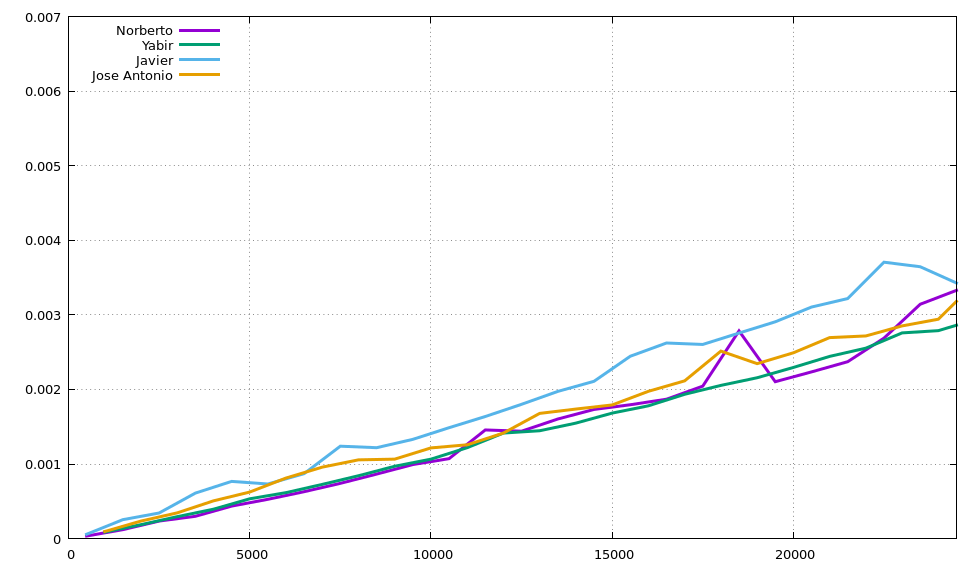
\includegraphics[width=0.8\textwidth]{../plots/quicksort}
	\caption{Comparativa de la eficiencia empírica del algoritmo $quicksort$.}
\end{figure}

\begin{table}[h]
	\centering
	\caption{Heapsort}
	\begin{tabular}{ | c | c  | c | c | c | }
		\hline
		Tama\~no & Jose Antonio & Yabir & Javier & Norberto\\
		\hline
		1000	&	0.000132	&	0.000124	&	8.4e-05	&	7.9e-05	\\
		2000	&	0.000255	&	0.000268	&	0.000271	&	0.000406	\\
		3000	&	0.000456	&	0.000422	&	0.00052	&	0.000716	\\
		4000	&	0.00066	&	0.000585	&	0.000691	&	0.000526	\\
		5000	&	0.000863	&	0.000748	&	0.000947	&	0.000689	\\
		6000	&	0.000986	&	0.00092	&	0.001139	&	0.000857	\\
		7000	&	0.001072	&	0.001085	&	0.001664	&	0.001057	\\
		8000	&	0.001196	&	0.001164	&	0.001972	&	0.001217	\\
		9000	&	0.001481	&	0.001303	&	0.001855	&	0.001698	\\
		10000	&	0.001664	&	0.00146	&	0.00178	&	0.001912	\\
		11000	&	0.001884	&	0.001627	&	0.0019	&	0.002133	\\
		12000	&	0.002017	&	0.001808	&	0.002024	&	0.001551	\\
		13000	&	0.00231	&	0.001986	&	0.002234	&	0.001741	\\
		14000	&	0.002296	&	0.00212	&	0.002421	&	0.001831	\\
		15000	&	0.002411	&	0.002294	&	0.002654	&	0.001931	\\
		16000	&	0.002687	&	0.002464	&	0.002998	&	0.002472	\\
		17000	&	0.002767	&	0.002641	&	0.003026	&	0.002658	\\
		18000	&	0.003095	&	0.002815	&	0.003222	&	0.002725	\\
		19000	&	0.00318	&	0.00305	&	0.003449	&	0.002751	\\
		20000	&	0.003568	&	0.003175	&	0.00356	&	0.002975	\\
		21000	&	0.0036	&	0.003364	&	0.003925	&	0.004273	\\
		22000	&	0.003762	&	0.003576	&	0.004304	&	0.003447	\\
		23000	&	0.003894	&	0.003686	&	0.004233	&	0.003695	\\
		24000	&	0.00414	&	0.003889	&	0.004508	&	0.003796	\\
		25000	&	0.004257	&	0.004078	&	0.005877	&	0.005502	\\
		\hline
	\end{tabular}
\end{table}

\begin{figure}[H]
	\centering
	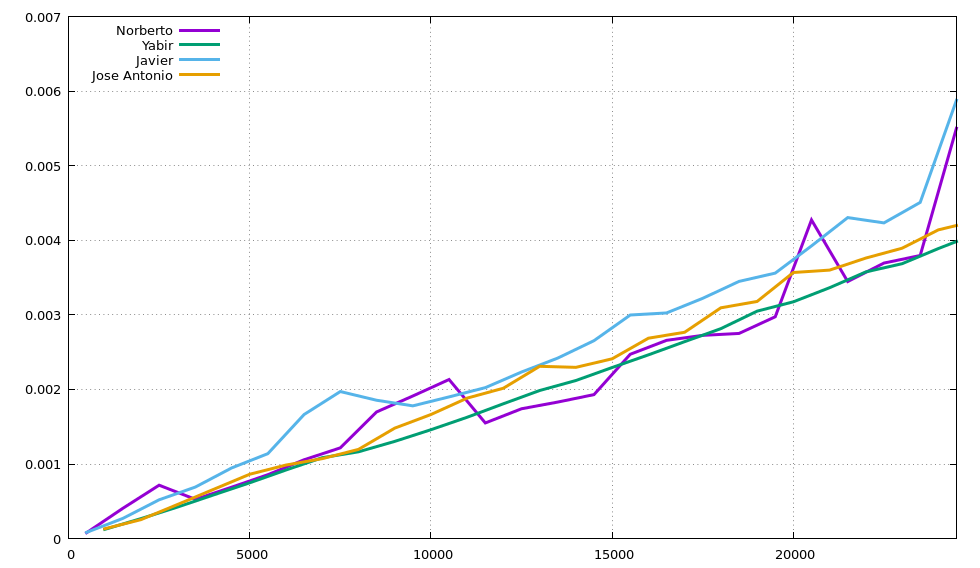
\includegraphics[width=0.8\textwidth]{../plots/heapsort}
	\caption{Comparativa de la eficiencia empírica del algoritmo $heapsort$.}
\end{figure}

\subsection{Algoritmo de orden cúbico}

Comencemos con el estudio teórico, manteniendo la notación utilizada hasta ahora. He aqui el algoritmo a estudiar, \textbf{floyd}:

\begin{lstlisting}
void Floyd(int **M, int dim) {
	for (int k = 0; k < dim; k++)
		for (int i = 0; i < dim;i++)
			for (int j = 0; j < dim;j++){
				int sum = M[i][k] + M[k][j];
				M[i][j] = (M[i][j] > sum) ? sum : M[i][j];
			}
}
\end{lstlisting}

$$\sum_{k=0}^{n} \sum_{i=0}^{n} \sum_{j=0}^{n} a = a n^3 \in O(n^3)$$

Tablas de datos y comparativa:

\begin{table}[h]
	\centering
	\caption{Floyd}
	\begin{tabular}{ | c | c  | c | c | c | }
		\hline
		Tama\~no & Jose Antonio & Yabir & Javier & Norberto\\
		\hline
		25	&	0.000106	&	0.000104	&	0.000132	&	0.000255	\\
		60	&	0.00132	&	0.001315	&	0.001638	&	0.00309	\\
		95	&	0.00529	&	0.005052	&	0.006333	&	0.009714	\\
		130	&	0.013483	&	0.012898	&	0.016173	&	0.013252	\\
		165	&	0.026949	&	0.025858	&	0.030908	&	0.023836	\\
		200	&	0.047713	&	0.046035	&	0.053756	&	0.040295	\\
		235	&	0.076571	&	0.074148	&	0.082185	&	0.064654	\\
		270	&	0.115361	&	0.111999	&	0.12578	&	0.097323	\\
		305	&	0.16553	&	0.161234	&	0.179741	&	0.141312	\\
		340	&	0.229901	&	0.223649	&	0.246866	&	0.194466	\\
		375	&	0.306628	&	0.303014	&	0.328515	&	0.258094	\\
		410	&	0.399503	&	0.38989	&	0.428172	&	0.337823	\\
		445	&	0.511245	&	0.497475	&	0.542359	&	0.430337	\\
		480	&	0.646562	&	0.624318	&	0.678628	&	0.5407	\\
		515	&	0.792583	&	0.76971	&	0.84846	&	0.667034	\\
		550	&	0.964084	&	0.936758	&	1.04872	&	0.812562	\\
		585	&	1.167	&	1.12769	&	1.23856	&	0.976406	\\
		620	&	1.39008	&	1.3435	&	1.45209	&	1.163	\\
		655	&	1.63592	&	1.57988	&	1.70619	&	1.36855	\\
		690	&	1.90257	&	1.84778	&	1.9882	&	1.60272	\\
		725	&	2.21537	&	2.13758	&	2.32022	&	1.85235	\\
		760	&	2.53784	&	2.46761	&	2.67501	&	2.13302	\\
		795	&	2.92257	&	2.84002	&	3.07144	&	2.44512	\\
		830	&	3.30624	&	3.23833	&	3.4851	&	2.78404	\\
		865	&	3.78033	&	3.65871	&	3.96119	&	3.15061	\\
		\hline
	\end{tabular}
\end{table}

\begin{figure}[H]
	\centering
	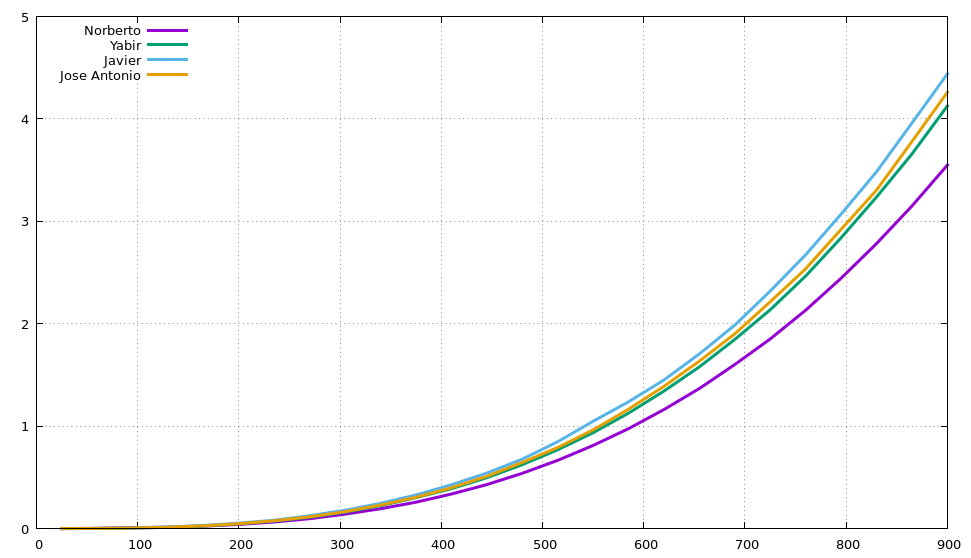
\includegraphics[width=0.8\textwidth]{../plots/floyd}
	\caption{Comparativa de la eficiencia empírica del algoritmo $floyd$.}
\end{figure}

\subsection{Algoritmo de orden exponencial}

Comencemos con el estudio teórico. He aqui el algoritmo a estudiar, \textbf{hanoi}:

\begin{lstlisting}
void hanoi (int M, int i, int j) {
	if (M > 0) {
		hanoi(M-1, i, 6-i-j);
		hanoi (M-1, 6-i-j, j);
	}
}
\end{lstlisting}

Como este algoritmo se llama a si mismo dos veces podemos expresar su eficiencia vara una entrada $n$ como:

$$Hanoi(n) = 2 \cdot Hanoi(n-1)$$

Viendo esta expresión como una ecuación en recurrencias:

$$X_{n+1} = 2 \cdot X_n$$

Esto es una progresión geométrica cuya solución viene expresada por:

$$X_n = C \cdot 2^n \in O(2^n)$$

Donde $C$ es una constante que depende del problema. Una vez finalizado el estudio teórico representamos los datos obtenidos junto con la comparativa pertinente:

\begin{table}[h]
	\centering
	\caption{Hanoi}
	\begin{tabular}{ | c | c  | c | c | c | }
		\hline
		Tama\~no & Jose Antonio & Yabir & Javier & Norberto\\
		\hline
		5	&	1e-06	&	2e-06	&	3e-06	&	4e-06	\\
		6	&	2e-06	&	1e-06	&	2e-06	&	6e-06	\\
		7	&	3e-06	&	2e-06	&	3e-06	&	2e-06	\\
		8	&	3e-06	&	3e-06	&	5e-06	&	2e-06	\\
		9	&	4e-06	&	4e-06	&	6e-06	&	4e-06	\\
		10	&	7e-06	&	7e-06	&	1.1e-05	&	8e-06	\\
		11	&	1.5e-05	&	1.4e-05	&	1.9e-05	&	1.3e-05	\\
		12	&	2.9e-05	&	2.7e-05	&	4.7e-05	&	2.5e-05	\\
		13	&	5.4e-05	&	5.3e-05	&	9.2e-05	&	5e-05	\\
		14	&	0.000107	&	0.000103	&	0.000152	&	9.7e-05	\\
		15	&	0.000212	&	0.000205	&	0.000257	&	0.000193	\\
		16	&	0.000422	&	0.000409	&	0.000473	&	0.000386	\\
		17	&	0.000844	&	0.000817	&	0.000923	&	0.000769	\\
		18	&	0.001684	&	0.001631	&	0.001819	&	0.001537	\\
		19	&	0.003403	&	0.00327	&	0.003653	&	0.003089	\\
		20	&	0.006931	&	0.006554	&	0.007464	&	0.005846	\\
		21	&	0.013697	&	0.01307	&	0.014864	&	0.015505	\\
		22	&	0.027919	&	0.027262	&	0.029788	&	0.023595	\\
		23	&	0.054677	&	0.052523	&	0.059037	&	0.046132	\\
		24	&	0.108517	&	0.104901	&	0.116334	&	0.091187	\\
		25	&	0.216675	&	0.209356	&	0.228908	&	0.181641	\\
		26	&	0.434431	&	0.417555	&	0.456383	&	0.362962	\\
		27	&	0.867205	&	0.83499	&	0.908195	&	0.725599	\\
		28	&	1.73855	&	1.6775	&	1.80609	&	1.45384	\\
		29	&	3.46495	&	3.35842	&	3.60959	&	2.9018	\\
		\hline
	\end{tabular}
\end{table}

\begin{figure}[H]
	\centering
	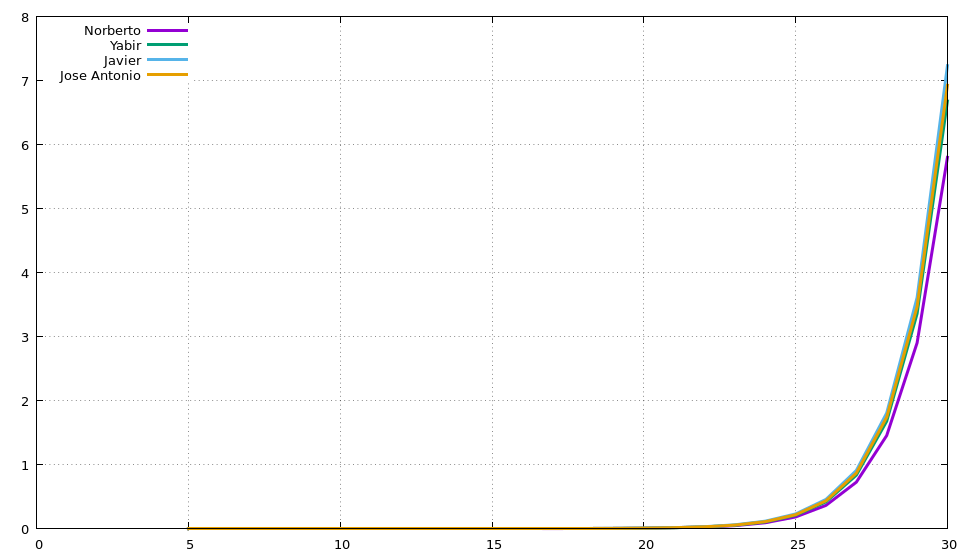
\includegraphics[width=0.8\textwidth]{../plots/hanoi}
	\caption{Comparativa de la eficiencia empírica del algoritmo $hanoi$.}
\end{figure}

\section{Conclusión}

Como hemos podido ir observando en las gráficas comparativas de los distintos algoritmos,
no importa el equipo que estemos utilizando para el estudio de estos, es decir,
independientemente de la velocidad de cálculo que tenga un ordenador u otro
el orden de los algoritmos no varía.

\end{document}
